%%%%%%%%%%%%%%%%%%%%% {{{
%%Options for presentations (in-class) and handouts (e.g. print).
\documentclass[pdf,9pt]{beamer}


%%%%%%%%%%%%%%%%%%%%%%
%Change this for different slides so it appears in bar
\usepackage{authoraftertitle}
\date{Chapter 8. Orthogonality \\ \S  8-1. Orthogonal Complements and Projections}

%%%%%%%%%%%%%%%%%%%%%%
%% Upload common style file
\usepackage{LyryxLAWASlidesStyle}

\begin{document}

%%%%%%%%%%%%%%%%%%%%%%%
%% Title Page and Copyright Common to All Slides

%Title Page
\input frontmatter/titlepage.tex

%LOTS Page
\input frontmatter/lyryxopentexts.tex

%Copyright Page
\input frontmatter/copyright.tex

%%%%%%%%%%%%%%%%%%%%%%%%% }}}
%-------------- start slide -------------------------------%{{{ 2
\begin{frame}[fragile]
   \tableofcontents
\end{frame}
%-------------- end slide -------------------------------%}}}
\section[\textcolor{yellow}{}]{\textcolor{yellow}{Orthogonal Bases}}
%-------------- start slide -------------------------------%{{{ 3
\frame{
\frametitle{Orthogonality Basis}
\pause
\begin{definition}[Orthogonality]
    \begin{itemize}
	\item Let $\vec{x},\vec{y}\in\RR^n$.  We say the $\vec{x}$ and $\vec{y}$ are \alert{orthogonal} if $\vec{x}\dotprod\vec{y}=0$.
	\item More generally,
	    $X=\{\vec{x}_1, \vec{x}_2, \ldots, \vec{x}_k\}\subseteq\RR^n$ is
	    an \alert{orthogonal set} if each $\vec{x_i}$ is
	    nonzero, and every pair of distinct vectors of $X$ is orthogonal, i.e.,
	    $\vec{x}_i\dotprod \vec{x}_j=0$ for all $i\neq j$,
	    $1\leq i,j\leq k$.
	\item A set
	    $X=\{\vec{x}_1, \vec{x}_2, \ldots, \vec{x}_k\}\subseteq\RR^n$ is
	    an \alert{orthonormal set} if $X$ is an orthogonal set of
	    unit vectors, i.e., $||\vec{x}_i||=1$ for
	    all $i$, $1\leq i\leq k$.
    \end{itemize}
\end{definition}
\vfill
\[\bigcap\]
\vfill
\begin{definition}[Linearly Independence]
    Let $V$ be a vector space and
    $S=\{\vec{x}_1, \vec{x}_2, \ldots, \vec{x}_k\}$ a subset of $V$.
    The set $S$ is \textcolor{lgtblue}{linearly independent} if the following condition holds:
    \[
	s_1\vec{x}_1 + s_2\vec{x}_2 +\cdots +s_k\vec{x}_k = \vec{0}
	\quad\Rightarrow\quad
	s_1=s_2=\cdots=s_k=0.
    \]
\end{definition}
}
%-------------- end slide -------------------------------%}}}
%-------------- start slide -------------------------------%{{{ 4
\frame{
\begin{lemma}[Independent Lemma]
    Let $V$ be a vector space and $S=\{ \bm{v}_1, \bm{v}_2, \ldots, \bm{v}_k\}$
    an \textcolor{lgtblue}{independent subset} of $V$.
    If $\bm{u}$ is a vector in $V$, but $\bm{u}\not\in\Span(S)$, then
    $S^{\prime}=\{ \bm{v}_1, \bm{v}_2, \ldots, \bm{v}_k, \bm{u}\}$ is independent.
\end{lemma}
\vfill
\[\text{--- v.s. ---}\]
\vfill
\begin{lemma}[Orthogonal Lemma]
    Suppose $\{ \vec{f}_1, \vec{f}_2, \ldots, \vec{f}_m\}$ is an
    \alert{orthogonal subset} of $\RR^n$, and suppose $\vec{x}\in\RR^n$.
    Define
    \[
      \vec{f}_{m+1}=\vec{x}
      -\frac{\vec{x}\dotprod\vec{f}_1}{||\vec{f}_1||^2}\vec{f}_1
      -\frac{\vec{x}\dotprod\vec{f}_2}{||\vec{f}_2||^2}\vec{f}_2 -\cdots
      -\frac{\vec{x}\dotprod\vec{f}_m}{||\vec{f}_m||^2}\vec{f}_m.
    \]
    Then
    \begin{enumerate}
	\item $\vec{f}_{m+1}\dotprod \vec{f}_j=0$ for all $j$, $1\leq j\leq m$.
	\item If $\vec{x}\not\in\Span\{ \vec{f}_1, \vec{f}_2, \ldots, \vec{f}_m\}$,
	    then $\vec{f}_{m+1} \neq \vec{0}$, and
	    $\{ \vec{f}_1, \vec{f}_2, \ldots, \vec{f}_m, \vec{f}_{m+1}\}$ is
	    an orthogonal set.
    \end{enumerate}
\end{lemma}
}
%-------------- end slide -------------------------------%}}}
%-------------- start slide -------------------------------%{{{ 5
\frame{
\begin{proofnoend}[of orthogonal lemma]
    (1) For any $1\le k\le m$
    \begin{align*}
    \vec{f}_{m+1}\cdot \vec{f}_k & = \left(\vec{x} -\frac{\vec{x}\dotprod\vec{f}_1}{||\vec{f}_1||^2}\vec{f}_1 -\frac{\vec{x}\dotprod\vec{f}_2}{||\vec{f}_2||^2}\vec{f}_2 -\cdots -\frac{\vec{x}\dotprod\vec{f}_m}{||\vec{f}_m||^2}\vec{f}_m\right) \cdot \vec{f}_k \\
    			     & = \vec{x}\cdot\vec{f}_k  -\frac{\vec{x}\dotprod\vec{f}_1}{||\vec{f}_1||^2}\vec{f}_1\cdot\vec{f}_k -\frac{\vec{x}\dotprod\vec{f}_2}{||\vec{f}_2||^2}\vec{f}_2\cdot\vec{f}_k -\cdots -\frac{\vec{x}\dotprod\vec{f}_m}{||\vec{f}_m||^2}\vec{f}_m\cdot\vec{f}_k \\
    			     & = \vec{x}\cdot\vec{f}_k  -\frac{\vec{x}\dotprod\vec{f}_k}{||\vec{f}_k||^2}\vec{f}_k\cdot\vec{f}_k\\
    			     & = \vec{x}\cdot\vec{f}_k  -\vec{x}\cdot\vec{f}_k = 0.
    \end{align*}
\end{proofnoend}
}
%-------------- end slide -------------------------------%}}}
%-------------- start slide -------------------------------%{{{ 6
\frame{
\begin{proofnoend}[continued]
    (2) Since $\{\vec{f}_1,\cdots,\vec{f}_m\}$ are independent, by the unique representation theorem,
    $\vec{x}\in\Span\{ \vec{f}_1, \vec{f}_2, \ldots, \vec{f}_m\}$, iff there exists unique representation for $\vec{x}$
    \begin{align*}
        \vec{x} = a_1 \vec{f}_1 + \cdots + a_m \vec{f}_m.
    \end{align*}
    Using the fact that $\{\vec{f}_1,\cdots,\vec{f}_m\}$ is orthogonal, one finds that
    \begin{align*}
	a_i = \frac{\vec{x}\cdot \vec{f}_i}{||\vec{f}_i||^2}.
    \end{align*}
    In other words,
    \begin{align*}
	\vec{x}\in \Span \{\vec{f}_1,\cdots,\vec{f}_m\} \quad\Longleftrightarrow\quad
	\vec{f}_{m+1}=\vec{x}
	-\frac{\vec{x}\dotprod\vec{f}_1}{||\vec{f}_1||^2}\vec{f}_1
	-\frac{\vec{x}\dotprod\vec{f}_2}{||\vec{f}_2||^2}\vec{f}_2 -\cdots
	-\frac{\vec{x}\dotprod\vec{f}_m}{||\vec{f}_m||^2}\vec{f}_m = \vec{0}.
    \end{align*}
    Now, $\vec{x}\not\in\Span\{\vec{f}_1,\cdots,\vec{f}_m\}$  implies that $\vec{f}_{m+1}\ne \vec{0}$. 
    \bigskip

    Finally, $\{ \vec{f}_1, \vec{f}_2, \ldots, \vec{f}_m, \vec{f}_{m+1}\}$ is orthogonal thanks to (1).
    \myQED
\end{proofnoend}
}
%-------------- end slide -------------------------------%}}}
%-------------- start slide -------------------------------%{{{ 7
\frame{
\begin{theorem}
    Let $U$ be a subspace of $\RR^n$.
    \begin{enumerate}
	\item Every orthogonal subset $\{ \vec{f}_1, \vec{f}_2, \ldots, \vec{f}_m\}$ of $U$ is a subset of an orthogonal basis of $U$.
	\item $U$ has an orthogonal basis.
    \end{enumerate}
\end{theorem}
% \pause
\vfill
\begin{proofnoend}
    % (1) Algorithm:
\begin{center}
    \begin{minipage}{0.75\textwidth}
	\begin{algorithm*}[H]
	\SetKwInOut{Input}{Input}\SetKwInOut{Output}{Output}
	\Input{An orthogonal set $\{ \vec{f}_1, \vec{f}_2, \ldots, \vec{f}_m\}\subseteq U\subseteq \R^n$}
	\BlankLine
	\SetAlgoLined
	 $m\to n$\;
	 \While{$\Span\{\vec{f}_1,\cdots,\vec{f}_n\}\ne U$}{
	   Pick up arbitrary $\vec{x}\in U\setminus \Span\{\vec{f}_1,\cdots,\vec{f}_n\}$\;
	   Let $\vec{f}_{n+1}$ be given by the Orthogonal Lemma\;
	   Then $\{\vec{f}_1,\cdots,\vec{f}_n,\vec{f}_{n+1}\}$ is an orthogonal set\;
	   $n+1\to n$\;
	 }
	 \Output{An orthogonal basis $\{\vec{f}_1,\cdots,\vec{f}_n\}$ of $U$}
	 \caption{Proof of part (1) of Theorem}
	\end{algorithm*}
    \end{minipage}
\end{center}

    (2) If $U=\{\vec{0} \}$, done. Otherwise, find an arbitrary nonzero vector in $u$ and run the
    algorithm in (1).
    \myQED
\end{proofnoend}
}
%-------------- end slide -------------------------------%}}}
%-------------- start slide -------------------------------%{{{ 8
\frame{
\begin{theorem}[Gram-Schmidt Orthogonalization Algorithm]
    Let $U$ be a subset of $\RR^n$ and let
    $\{\vec{x}_1, \vec{x}_2, \ldots, \vec{x}_m\}$
    be a basis of $U$.
    Let $\vec{f}_1=\vec{x}_1$,
    and for each $j$, $2\leq j\leq m$, let
    \[
        \vec{f}_j=\vec{x}_j
    -\frac{\vec{x}_j\dotprod\vec{f}_1}{||\vec{f}_1||^2}\vec{f}_1
    -\frac{\vec{x}_j\dotprod\vec{f}_2}{||\vec{f}_2||^2}\vec{f}_2 -\cdots
    -\frac{\vec{x}_j\dotprod\vec{f}_{j-1}}{||\vec{f}_{j-1}||^2}\vec{f}_{j-1}.
    \]
    Then
    $\{ \vec{f}_1, \vec{f}_2, \ldots, \vec{f}_m\}$ is an
    orthogonal basis of $U$,
    and
    \[
      \Span\{ \vec{f}_1, \vec{f}_2, \ldots, \vec{f}_j\}=
      \Span\{ \vec{x}_1, \vec{x}_2, \ldots, \vec{x}_j\} \quad \forall j=1,\cdots,m.
    \]
\end{theorem}
}
%-------------- end slide -------------------------------%}}}
%-------------- start slide -------------------------------%{{{ 9
\frame{
\begin{emptytitle}
\begin{center}
	\begin{minipage}{0.85\textwidth}
	    \begin{algorithm*}[H]
	    \SetKwInOut{Input}{Input}\SetKwInOut{Output}{Output}
	    \Input{A basis $\{ \vec{x}_1, \vec{x}_2, \ldots, \vec{x}_m\}\subseteq U\subseteq \R^n$}
	    \BlankLine
	    \SetAlgoLined
	    $\vec{f}_1\leftarrow \vec{x}_1$\;
	     \For{$j\leftarrow 2$ \KwTo $m$}{
           \[
                \vec{f}_j\leftarrow \vec{x}_j
            -\frac{\vec{x}_j\dotprod\vec{f}_1}{||\vec{f}_1||^2}\vec{f}_1
            -\frac{\vec{x}_j\dotprod\vec{f}_2}{||\vec{f}_2||^2}\vec{f}_2 -\cdots
            -\frac{\vec{x}_j\dotprod\vec{f}_{j-1}}{||\vec{f}_{j-1}||^2}\vec{f}_{j-1}.
           \]
	     }
       \Output{An orthogonal basis $\{\vec{f}_1,\cdots,\vec{f}_m\}$ of $U$ s.t.\\
          $\Span\{ \vec{f}_1, \vec{f}_2, \ldots, \vec{f}_j\}= \Span\{ \vec{x}_1, \vec{x}_2, \ldots, \vec{x}_j\}$\\
          for all $j=1,\cdots,m$.
        }
	     \caption{Gram-Schmidt Orthogonalization Algorithm}
	    \end{algorithm*}
	\end{minipage}
\end{center}
\end{emptytitle}
}
%-------------- end slide -------------------------------%}}}
%-------------- start slide -------------------------------%{{{ 10
\frame{
\[
    \begin{array}{ccc}
        \Span \{\vec{a}_1,\vec{a}_2,\vec{a}_3  \} & =   & \Span \{\vec{b}_1,\vec{b}_2,\vec{b}_3\} \\ [1em]
        \text{basis}                              & \to & \text{orthogonal basis}
    \end{array}
\]
\vfill
\begin{center}
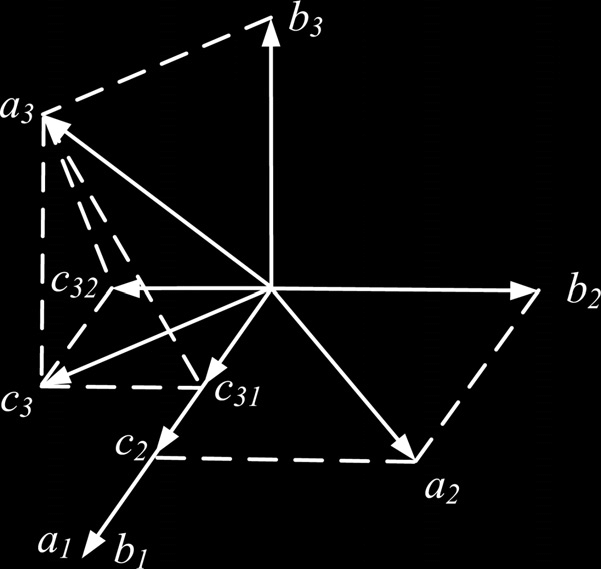
\includegraphics[scale=0.23]{./figures/An-illustration-of-Gram-Schmidt-transformation-neg.png}
\end{center}
}
%-------------- end slide -------------------------------%}}}
%-------------- start slide -------------------------------%{{{ 11
\frame{
\begin{problem}
    Let
    \[
	\vec{x}_1=\left[\begin{array}{c} 1\\ 0\\ 1\\ 0 \end{array}\right], \quad
	\vec{x}_2=\left[\begin{array}{c} 1\\ 0\\ 1\\ 1 \end{array}\right], \quad\text{and}\quad
	\vec{x}_3=\left[\begin{array}{c} 1\\ 1\\ 0\\ 0 \end{array}\right],
    \]
    and let $U=\Span\{\vec{x}_1, \vec{x}_2,\vec{x}_3\}$.
    We use the Gram-Schmidt Orthogonalization Algorithm
    to construct an orthogonal basis $B$ of $U$.
\end{problem}
\pause
\vfill
\begin{proofnoend}
    First $\vec{f}_1=\vec{x}_1$.
    \pause
    Next,
    \[ \vec{f}_2=\left[\begin{array}{c} 1\\ 0\\ 1\\ 1 \end{array}\right]
    -\frac{2}{2}\left[\begin{array}{c} 1\\ 0\\ 1\\ 0 \end{array}\right]
    =\left[\begin{array}{c} 0\\ 0\\ 0\\ 1 \end{array}\right].\]
    \pause
    Finally,
    \[ \vec{f}_3=\left[\begin{array}{c} 1\\ 1\\ 0\\ 0 \end{array}\right]
    -\frac{1}{2}\left[\begin{array}{c} 1\\ 0\\ 1\\ 0 \end{array}\right]
    -\frac{0}{1}\left[\begin{array}{c} 0\\ 0\\ 0\\ 1 \end{array}\right]
    =\left[\begin{array}{c} 1/2\\ 1\\ -1/2\\ 0 \end{array}\right].\]
\end{proofnoend}
}
%-------------- end slide -------------------------------%}}}
%-------------- start slide -------------------------------%{{{ 12
\frame{
\begin{proofnoend}[continued]
    Therefore,
    \[ \left\{
	\left[\begin{array}{c} 1\\   0\\ 1\\    0 \end{array}\right],
	\left[\begin{array}{c} 0\\   0\\ 0\\    1 \end{array}\right],
	\left[\begin{array}{c} 1/2\\ 1\\ -1/2\\ 0 \end{array}\right]
    \right\}\]
    is an orthogonal basis of $U$.
    However, it is sometimes more convenient to deal with vectors
    having integer entries, in which case we take
    \[ B=\left\{
	\left[\begin{array}{c} 1\\ 0\\ 1\\  0 \end{array}\right],
	\left[\begin{array}{c} 0\\ 0\\ 0\\  1 \end{array}\right],
	\left[\begin{array}{r} 1\\ 2\\ -1\\ 0 \end{array}\right]
    \right\}.\]
    (Orthogonality of the set is not affected by multiplying vectors
    in the set by nonzero scalars.)
    \myQED
\end{proofnoend}
}
%-------------- end slide -------------------------------%}}}
\section[\textcolor{yellow}{}]{\textcolor{yellow}{The Orthogonal Complement $U^\perp$}}
%-------------- start slide -------------------------------%{{{ 13
\frame{
\frametitle{The Orthogonal Complement $U^\perp$}
\pause
\begin{definition}
    Let $U$ be a subspace of $\RR^n$.
    The \alert{orthogonal complement} of $U$, called \alert{$U$ perp},
    is denoted $U^{\perp}$ and is defined as
    \[ U^{\perp} = \{ \vec{x}\in\RR^n ~|~ \vec{x}\dotprod\vec{y}=0 \mbox{ for all } \vec{y}\in U\}.\]
\end{definition}
\pause
\vfill
\begin{center}
    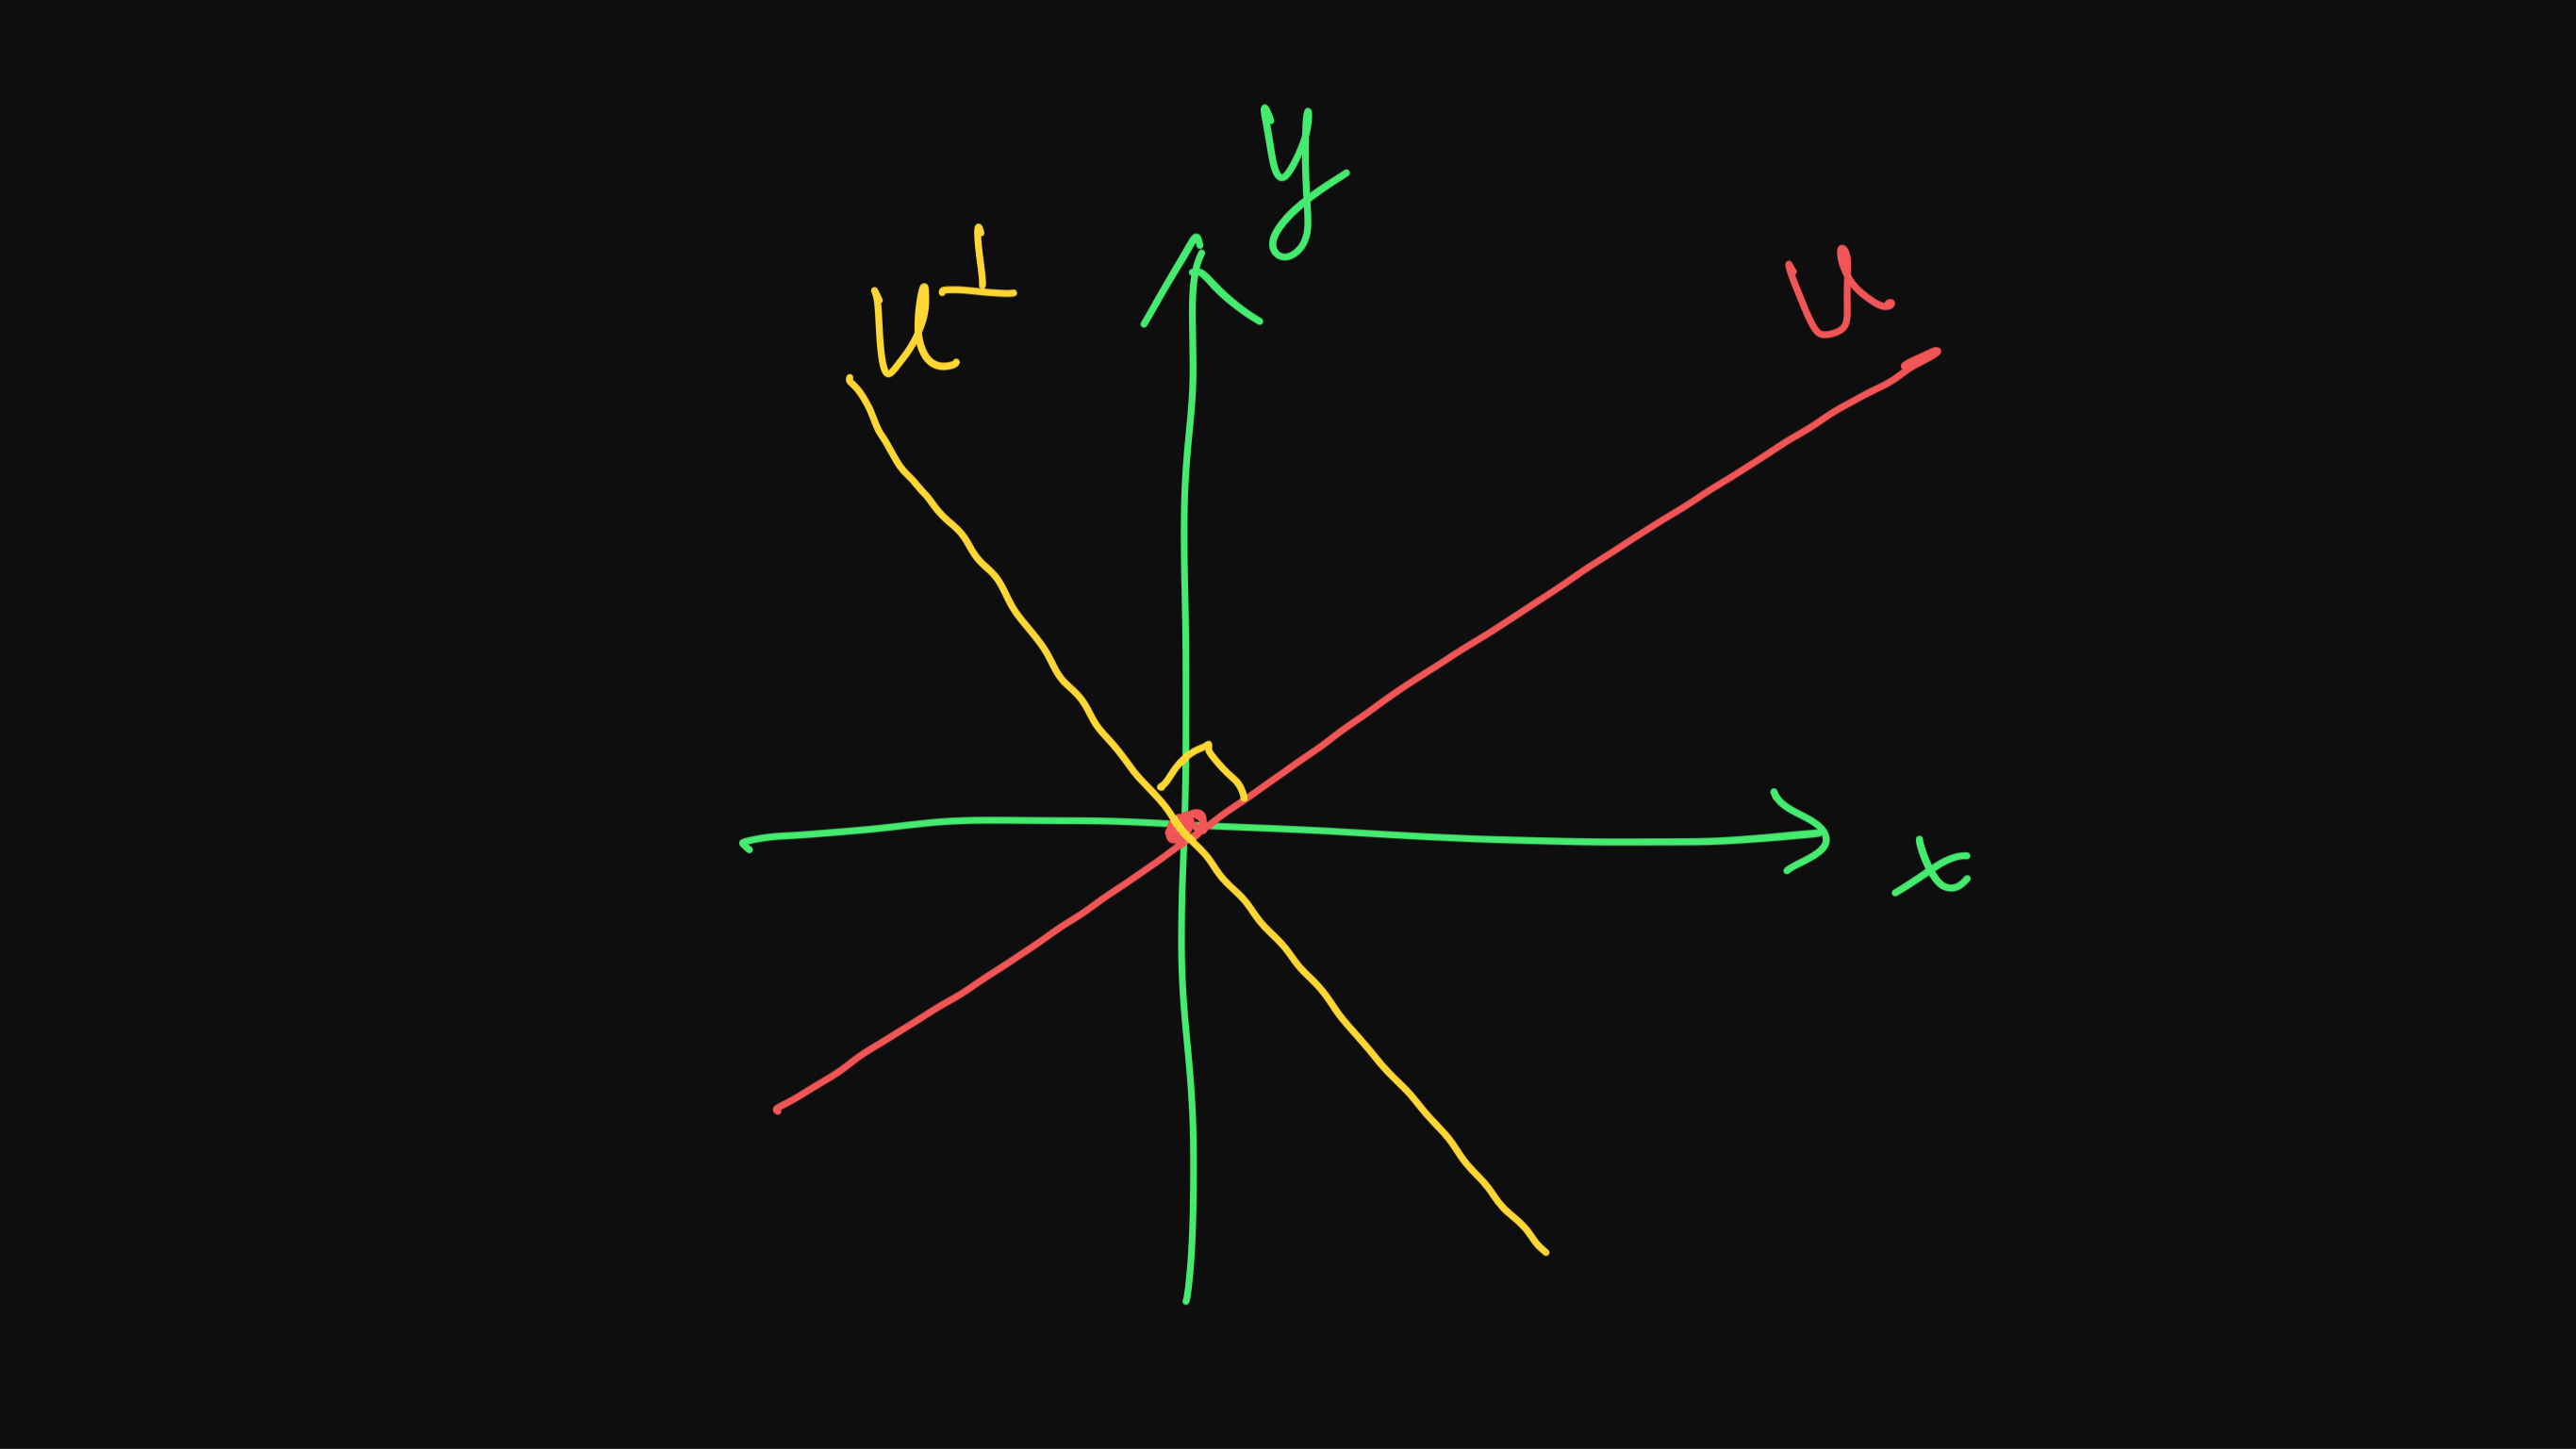
\includegraphics[scale=0.054]{./figures/Uperp/2d.png}
    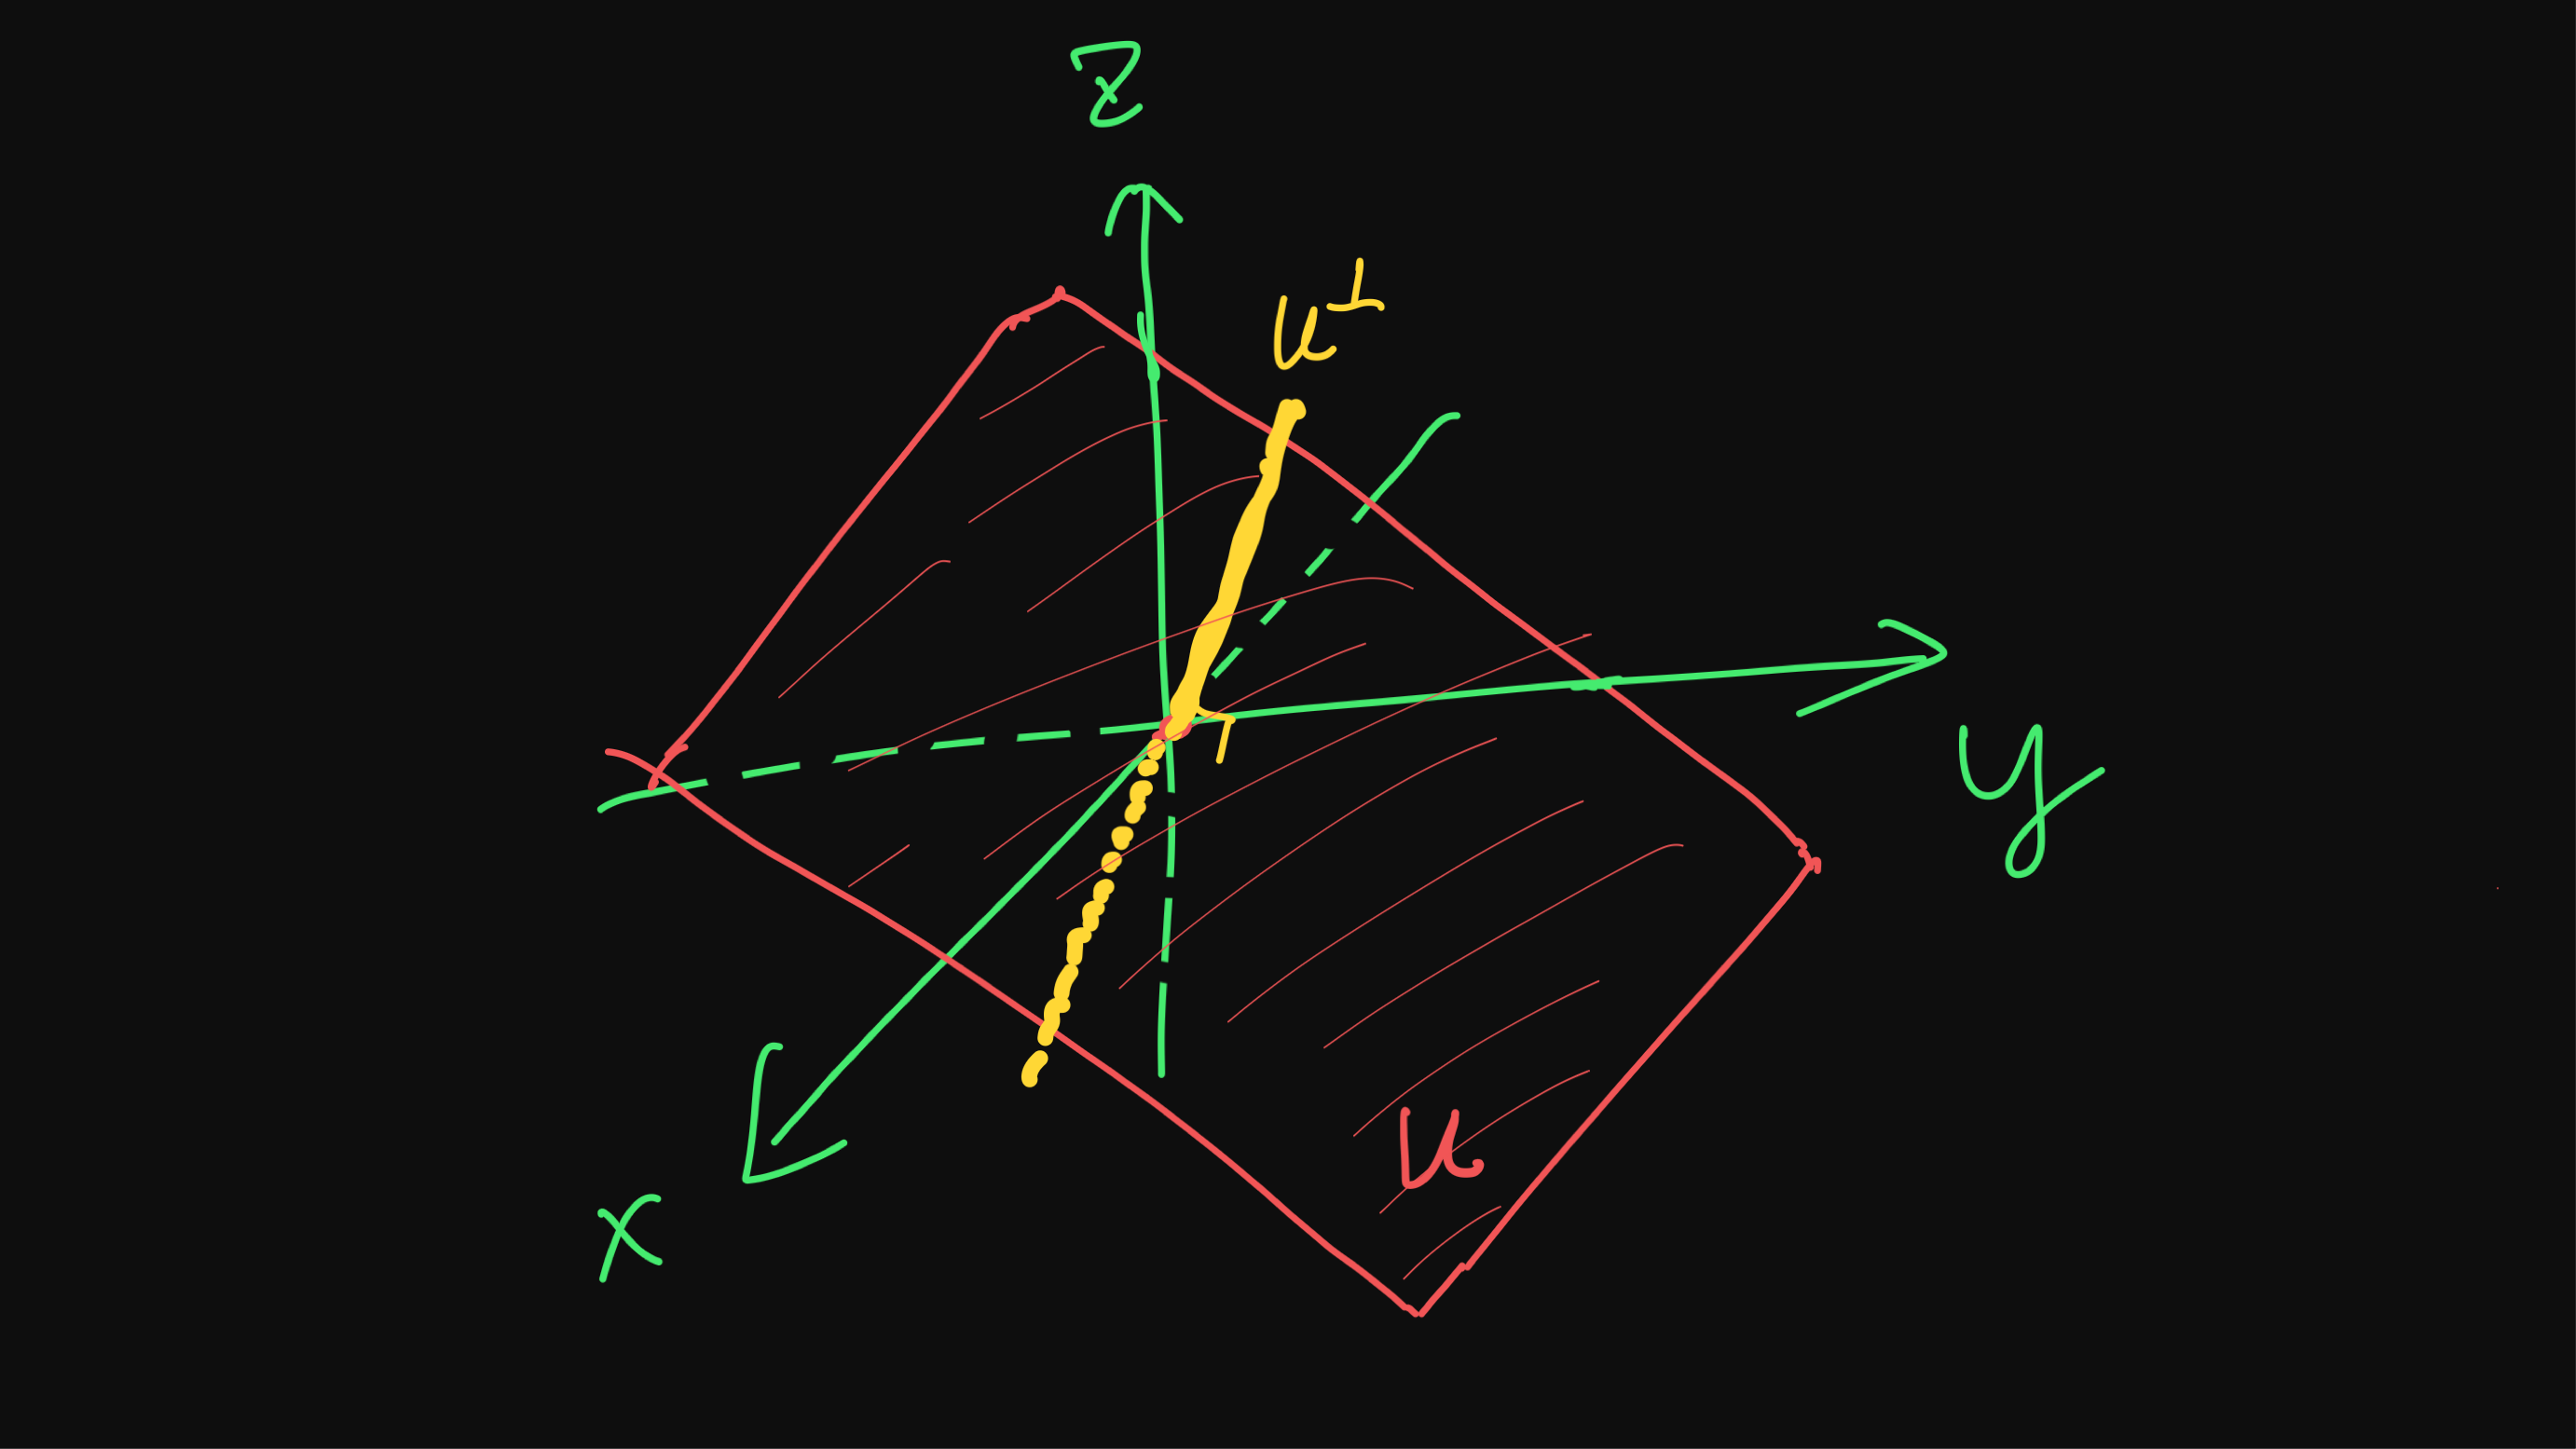
\includegraphics[scale=0.054]{./figures/Uperp/3d.png}
\end{center}
}
%-------------- end slide -------------------------------%}}}
%-------------- start slide -------------------------------%{{{ 14
\frame{
\begin{example}
    Let $U=\Span\left\{
	\left[\begin{array}{r} -2 \\ 3  \\ 1 \end{array}\right],
	\left[\begin{array}{r} 5  \\ -1 \\ 2 \end{array}\right]\right\}$, and suppose
    $\vec{v}=\left[\begin{array}{r}  a \\ b \\ c \end{array}\right] \in U^{\perp}$.
    Then
    \[ -2a + 3b +c = 0 \quad\text{and}\quad 5a -b +2c = 0.\]
    This system of two equations in three variables has solution
    \begin{align*}
        \vec{v} = \begin{bmatrix} -7\\ -9\\ 13 \end{bmatrix} t,\quad\forall t\in\R,
    \end{align*}
    which is noting but a line passing through origin and perpendicular with the plane $U$.
\end{example}
}
%-------------- end slide -------------------------------%}}}
%-------------- start slide -------------------------------%{{{ 15
\frame{
\begin{theorem}[Properties of the Orthogonal Complement]
    Let $U$ be a subspace of $\RR^n$.
    \begin{enumerate}
	\item $U^{\perp}$ is a subspace of $\RR^n$.
	\item $\{ \vec{0}\}^{\perp}=\RR^n$ and $(\RR^n)^{\perp}=\{ \vec{0}\}$.
	\item If $U=\Span\{ \vec{y}_1, \vec{y}_2, \ldots, \vec{y}_m\}$,
	    then \[ U^{\perp} = \{ \vec{x}\in\RR^n ~|~ \vec{x}\dotprod\vec{y}_j=0 \mbox{ for } j=1,2,\ldots,m\}.\]
    \end{enumerate}
\end{theorem}
\pause
\vfill
\begin{proofnoend}
\begin{enumerate}
    \item This is a standard subspace proof and is left as an exercise.
    \pause
    \bigskip
    \item Here, $\vec{0}$ is the zero vector of $\RR^n$.  Since $\vec{x}\dotprod\vec{0}=0$ for all
	$\vec{x}\in\RR^n$, $\RR^n\subseteq\{ \vec{0}\}^{\perp}$.  Since $\{
	\vec{0}\}^{\perp}\subseteq\RR^n$, the equality follows, i.e., $\{ \vec{0}\}^{\perp}=\RR^n$.
	\bigskip

	Again, since $\vec{x}\dotprod\vec{0}=0$ for all $\vec{x}\in\RR^n$,
	$\vec{0}\in (\RR^n)^{\perp}$, so $\{ \vec{0}\}\subseteq(\RR^n)^{\perp}$.
	Suppose $\vec{x}\in\RR^n$, $\vec{x}\neq\vec{0}$.
	Since $\vec{x}\dotprod\vec{x}=||\vec{x}||^2$ and $\vec{x}\neq\vec{0}$,
	$\vec{x}\dotprod\vec{x}\neq 0$, so $\vec{x}\not\in(\RR^n)^{\perp}$.
	Therefore, $\{\vec{0}\}^c\subseteq \left((\RR^n)^{\perp}\right)^c$, or equivalently, $(\RR^n)^{\perp}\subseteq \{\vec{0}\}$.
	Thus $(\RR^n)^{\perp}=\{\vec{0}\}$.
\end{enumerate}
\end{proofnoend}
}
%-------------- end slide -------------------------------%}}}
%-------------- start slide -------------------------------%{{{ 16
\frame{
\begin{proofnoend}[continued]
\begin{enumerate}
    \setcounter{enumi}{2}
    \item Let $X= \{ \vec{x}\in\RR^n ~|~ \vec{x}\dotprod\vec{y}_j=0
	\mbox{ for } j=1,2,\ldots,m\}$.
  \bigskip

	``$U^{\perp}\subseteq X$'': ~Suppose that $\vec{v}\in U^{\perp}$.
	Then $\vec{v}$ is orthogonal to every vector in $U$;
	in particular, $\vec{v}\dotprod \vec{y}_j=0$ for $j=1,2,\ldots,m$
	since each such $\vec{y}_j$ is in $U$.
	Therefore, $\vec{v}\in X$. This proves that $U^{\perp}\subseteq X$.
  \bigskip
	\pause

	``$X \subseteq U^{\perp}$'': Now suppose that $\vec{v}\in X$ and $\vec{u}\in U$.
	Then $\vec{u}=a_1\vec{y}_1 + a_2\vec{y}_2 + \cdots + a_m\vec{y}_m$
	for some $a_1, a_2, \ldots, a_m\in\RR$, and so
	\begin{eqnarray*}
	\vec{v}\dotprod\vec{u}
	& = & \vec{v}\dotprod (a_1\vec{y}_1 + a_2\vec{y}_2 + \cdots + a_m\vec{y}_m) \\
	& = & \vec{v}\dotprod (a_1\vec{y}_1) + \vec{v}\dotprod(a_2\vec{y}_2) +
	\cdots + \vec{v}\dotprod(a_m\vec{y}_m) \\
	& = & a_1(\vec{v}\dotprod\vec{y}_1) +a_2(\vec{v}\dotprod\vec{y}_2) +
	\cdots + a_m(\vec{v}\dotprod\vec{y}_m).
	\end{eqnarray*}
	Since $\vec{v}\in X$, $\vec{v}\dotprod\vec{y}_j=0$ for all $j$,
	$1\leq j\leq m$.
	Therefore, $\vec{v}\dotprod\vec{u}=0$, and thus $X\subseteq U^{\perp}$.
	\pause
  \bigskip

	Finally, since $U^{\perp}\subseteq X$ and $X\subseteq U^{\perp}$, we see that $U^{\perp}=X$.
	\myQED
\end{enumerate}
\end{proofnoend}
}
%-------------- end slide -------------------------------%}}}
%-------------- start slide -------------------------------%{{{ 17
\frame{
\begin{problem}
    Let
    \[ U = \Span\left\{
	\left[\begin{array}{r} 0 \\ -1 \\ 3\\ 2 \end{array}\right],
	\left[\begin{array}{r} 2 \\ 1  \\ 0\\ 4 \end{array}\right] \right\}.\]
  Find $U^{\perp}$ by finding a basis of $U^\perp$.
\end{problem}
\pause
\begin{solution}
    \[ U^{\perp}=\left\{
      \left[ \left.\begin{array}{c} a\\b\\c\\d\end{array}\right]\in\RR^4 ~\right|~
    \left[\begin{array}{c} a\\b\\c\\d\end{array}\right] \dotprod
    \left[\begin{array}{r} 0 \\ -1 \\ 3\\ 2 \end{array}\right] =0 \quad\text{and}\quad
    \left[\begin{array}{c} a\\b\\c\\d\end{array}\right] \dotprod
    \left[\begin{array}{r} 2 \\ 1 \\ 0\\ 4 \end{array}\right]=0 \right\}.\]
      This leads to the system of two equation in four variables
      \begin{eqnarray*}
	-b+3c+2d & = & 0 \\
	2a+b+4d  & = & 0
      \end{eqnarray*}
\end{solution}
}
%-------------- end slide -------------------------------%}}}
%-------------- start slide -------------------------------%{{{ 18
\frame{
\begin{solution}[continued]
  \[ \uncover<2>{\alert{A=}}\left[\begin{array}{rrrr|r}
    0 & -1 & 3 & 2 & 0 \\
    2 & 1  & 0 & 4 & 0
    \end{array}\right]
  \rightarrow \cdots \rightarrow
  \left[\begin{array}{rrrr|r}
    1 & 0 & 3/2 & 3  & 0 \\
    0 & 1 & -3  & -2 & 0
    \end{array}\right]\]
  Therefore,
  \[ U^{\perp}=\left\{
    \left[ \left.\begin{array}{c}
    -\frac{3}{2}s - 3t\\
    3s+2t\\
  s\\t\end{array}\right]\in\RR^4
    ~\right|~ s,t\in\RR\right\}
    =
    \Span\left\{
  \left[\begin{array}{r}
  -\frac{3}{2}\\ 3\\ 1\\0\end{array}\right],
  \left[\begin{array}{c}
    3\\ 2\\ 0\\1\end{array}\right] \right\}.
\]
Since the set
$B=\left\{ \left[\begin{array}{r}
    -\frac{3}{2}\\ 3\\ 1\\0\end{array}\right],
    \left[\begin{array}{c}
3\\ 2\\ 0\\1\end{array}\right] \right\}$
is independent and spans $U^{\perp}$,
$B$ is a basis of $U^{\perp}$.
\myQED
\end{solution}
\vfill
\pause
\begin{remark}
    Notice that $U^{\perp}=\nul(A)$, where $A$ is the matrix
    whose rows are a spanning subset of $U$.
\end{remark}
}
%-------------- end slide -------------------------------%}}}
\section[\textcolor{yellow}{}]{\textcolor{yellow}{Definition of Orthogonal Projection}}
%-------------- start slide -------------------------------%{{{ 19
\frame{
\frametitle{Definition of Orthogonal Projection}
\pause
\begin{theorem}[Projection Formula]
    Suppose $\vec{u}$ and $\vec{v}$ are vectors in $\RR^3$,
    $\vec{v}\neq\vec{0}$.
    Then the \alert{projection of $\vec{u}$ on $\vec{v}$}, denoted as
    $\proj_{\vec{v}}(\vec{u})$, is equal to
    \[ \proj_{\vec{v}}(\vec{u}) =
    \left(\frac{\vec{u} \dotprod \vec{v}}{||\vec{v}||^2}\right) \vec{v}.\]
\end{theorem}
\vfill
\begin{center}
    \begin{picture}(4,1.0)
	\put(0.3,0.2){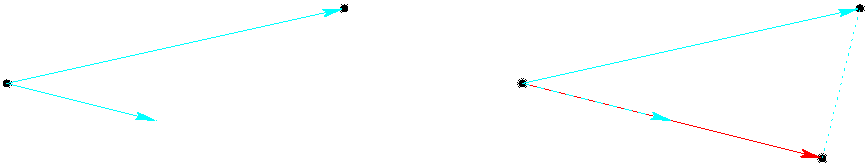
\includegraphics[scale=.7]{figures/projection_copy.pdf}}
	\put(1.0,0.8){\footnotesize $\vec{u}$}
	\put(0.6,0.32){\footnotesize $\vec{v}$}
	\put(3.35,0.8){\footnotesize $\vec{u}$}
	\put(3.2,0.2){\small \alert{$\proj_{\vec{v}}(\vec{u})$}}
    \end{picture}
\end{center}
}
%-------------- end slide -------------------------------%}}}
%-------------- start slide -------------------------------%{{{ 20
\begin{frame}[fragile]
  \begin{proofnoend}
  Let $\vec{p}= \proj_{\vec{v}}(\vec{u})$;
  then $\vec{p}$ is parallel to $\vec{v}$,
  so $\vec{p}=t\vec{v}$ for some $t\in\RR$,
  and $\vec{u}-\vec{p}=\vec{u}-t\vec{v}$ is orthogonal to $\vec{v}$, so
  \begin{eqnarray*}
  (\vec{u}-t\vec{v})\dotprod\vec{v} & = & 0 \\
  \vec{u}\dotprod\vec{v}-t\vec{v}\dotprod\vec{v} & = & 0 \\
  \vec{u}\dotprod\vec{v} & = & t||\vec{v}||^2
  \end{eqnarray*}
  \pause
  Since $\vec{v}\neq\vec{0}$,
  \[ t=\frac{\vec{u}\dotprod\vec{v}}{||\vec{v}||^2}.\]
  Therefore,
  \[ \vec{p}=t\vec{v}=
  \left(\frac{\vec{u}\dotprod\vec{v}}{||\vec{v}||^2}\right) \vec{v}.\]
  \myQED
 \end{proofnoend}
\end{frame}
%-------------- end slide -------------------------------%}}}
%-------------- start slide -------------------------------%{{{ 21
\frame{
\begin{remark}
  Note that
  \begin{itemize}
      \item $\{ \vec{v}\}$ is {an orthogonal basis} of the subspace
    $U$ of $\RR^3$ consisting of the line through the origin parallel
    to $\vec{v}$.
      \item $\vec{u}-\vec{p}\in U^{\perp}$
    (since $(\vec{u}-\vec{p})\dotprod\vec{v}=0$).
  \end{itemize}
\end{remark}
}
%-------------- end slide -------------------------------%}}}
%-------------- start slide -------------------------------%{{{ 22
\frame{
  \begin{example}[ Generalizing to $\RR^n$ ]
    Suppose $U$ is a subspace of $\RR^n$, $\vec{x}\in\RR^n$,
    and that
    $\{ \vec{f}_1, \vec{f}_2, \ldots, \vec{f}_m\}$ and
    $\{ \vec{g}_1, \vec{g}_2, \ldots, \vec{g}_m\}$
    are orthogonal bases of $U$.
    Define
    \begin{align*}
        \vec{p}_f & =
        \left(\frac{\vec{x}\dotprod\vec{f}_1}{||\vec{f}_1||^2}\right)\vec{f}_1
        +\left(\frac{\vec{x}\dotprod\vec{f}_2}{||\vec{f}_2||^2}\right)\vec{f}_2
        +\cdots
        +\left(\frac{\vec{x}\dotprod\vec{f}_m}{||\vec{f}_m||^2}\right)\vec{f}_m
        ~\mbox{ and}\\
        \vec{p}_g & =
        \left(\frac{\vec{x}\dotprod\vec{g}_1}{||\vec{g}_1||^2}\right)\vec{g}_1
        +\left(\frac{\vec{x}\dotprod\vec{g}_2}{||\vec{g}_2||^2}\right)\vec{g}_2
        +\cdots
        +\left(\frac{\vec{x}\dotprod\vec{g}_m}{||\vec{g}_m||^2}\right)\vec{g}_m.
    \end{align*}
    \pause
    Then $\vec{p}_f, \vec{p}_g\in U$ (since they are linear combinations of
    vectors of $U$) and
    $\vec{x}-\vec{p}_f,\vec{x}-\vec{p}_g\in U^{\perp}$ (by the
    {\bf Orthogonal Lemma}).
    \pause
    This implies that
    $\vec{p}_f - \vec{p}_g\in U$, and
    $(\vec{x}-\vec{p}_g) -(\vec{x}-\vec{p}_f)\in U^{\perp}$.
    However,
    \[ (\vec{x}-\vec{p}_g) -(\vec{x}-\vec{p}_f)  =
    \vec{p}_f - \vec{p}_g,\]
    and thus $\vec{p}_f - \vec{p}_g$ is in both $U$ and
    $U^{\perp}$.
    This is possible if and only if $\vec{p}_f - \vec{p}_g=\vec{0}$,
    i.e., $\vec{p}_f = \vec{p}_g$.
    \alert{This means that the computation of  $\vec{p}_f$ and
        $\vec{p}_g$ does not depend on which orthogonal basis is
    used.}
  \end{example}
}
%-------------- end slide -------------------------------%}}}
%-------------- start slide -------------------------------%{{{ 23
\frame{
\begin{definition}
    Let $\{\vec{f}_1, \vec{f}_2, \ldots, \vec{f}_m\}$ be an orthogonal
    basis for a subspace $U$ of $\RR^n$,
    and let $\vec{x}\in\RR^n$.
    The \alert{projection of $\vec{x}$ on $U$} is defined as
    \[ \proj_U(\vec{x}) =
      \left(\frac{\vec{x}\dotprod\vec{f}_1}{||\vec{f}_1||^2}\right)\vec{f}_1
      +\left(\frac{\vec{x}\dotprod\vec{f}_2}{||\vec{f}_2||^2}\right)\vec{f}_2
      +\cdots
    +\left(\frac{\vec{x}\dotprod\vec{f}_m}{||\vec{f}_m||^2}\right)\vec{f}_m.\]
\end{definition}
\vfill
\pause
\begin{remark}
\begin{enumerate}
    \item if $U=\{\vec{0}\}$, then $\proj_{\{\vec{0}\}}(\vec{x})= \vec{0}$ for any $\vec{x}\in\RR^n$;
    \item if $\vec{x}\in U$, then $\proj_U(\vec{x})$ is also called the \textcolor{red}{Fourier Expansion} of $\vec{x}$.
    \item In Orthogonal Lemma
        \begin{align*}
          \vec{f}_{m+1}=\vec{x}
          -\underbrace{\left(\frac{\vec{x}\dotprod\vec{f}_1}{||\vec{f}_1||^2}\vec{f}_1
          +\frac{\vec{x}\dotprod\vec{f}_2}{||\vec{f}_2||^2}\vec{f}_2 -\cdots
          +\frac{\vec{x}\dotprod\vec{f}_m}{||\vec{f}_m||^2}\vec{f}_m\right)}_{\displaystyle =\proj_U(\vec{x})}.
        \end{align*}
\end{enumerate}
\end{remark}
}
%-------------- end slide -------------------------------%}}}
\section[\textcolor{yellow}{}]{\textcolor{yellow}{The Projection Theorem and its Implications}}
%-------------- start slide -------------------------------%{{{ 24
\frame{
\frametitle{The Projection Theorem and its Implications}
\pause
\begin{theorem}[Projection Theorem]
    Let $U$ be a subspace of $\RR^n$, $\vec{x}\in\RR^n$, and \textcolor{blue}{$\vec{p}=\proj_U(\vec{x})$}.
    Then
    \begin{enumerate}
        \item $\textcolor{blue}{\vec{p}}\in U$ and $\textcolor{red}{\vec{x}-\vec{p}}\in U^{\perp}$;
        \item $\textcolor{blue}{\vec{p}}$ is the vector in $U$ closest to $\vec{x}$, meaning that for any $\vec{y}\in U$, $\vec{y}\neq \vec{p}$, \[ ||\vec{x}-\vec{p}|| < ||\vec{x}-\vec{y}||.\]
    \end{enumerate}
\end{theorem}
\pause
\vfill
\begin{center}
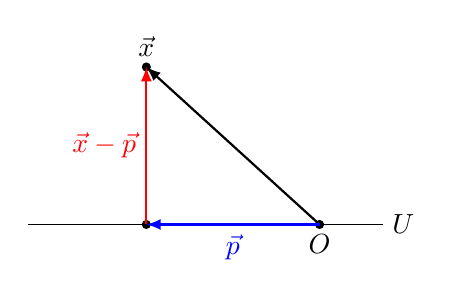
\begin{tikzpicture}[scale=1, transform shape]
    \tikzset{>=latex}
    \coordinate (P) at (1,3);
    \coordinate (Q) at (3.2,1);
    \coordinate (N) at (1,1);
    % \draw (0,0) -- (1.2, 2) -- (3.7,2) -- (3,0) -- (0,0);
    \draw (-0.5,1) -- (4,1) node [right] {$U$};
    \draw[<-,thick] (P) node [above] {$\vec{x}$} -- (Q) node [below] {$O$};
    \filldraw (P) circle (0.05);
    \filldraw (Q) circle (0.05);
    \filldraw (N) circle (0.05);
    \draw [blue,->,thick] (Q) -- (N) node[midway,below] {$\vec{p} $};
    \draw [red,->,thick] (N) -- (P) node[midway,left] {$\vec{x} - \vec{p} $};
\end{tikzpicture}
\qquad
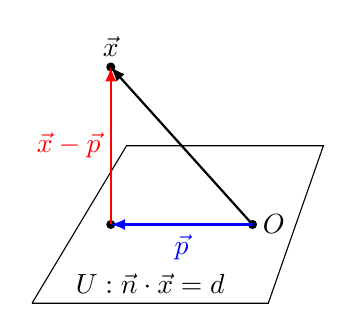
\begin{tikzpicture}[scale=1, transform shape]
    \tikzset{>=latex}
    \coordinate (P) at (1,3);
    \coordinate (Q) at (2.8,1);
    \coordinate (N) at (1,1);
    \draw (0,0) -- (1.2, 2) -- (3.7,2) -- (3,0) -- (0,0);
    \draw[<-,thick] (P) node [above] {$\vec{x}$} -- (Q) node [right] {$O$};
    \filldraw (P) circle (0.05);
    \filldraw (Q) circle (0.05);
    \filldraw (N) circle (0.05);
    \draw [blue,->,thick] (Q) -- (N) node[midway,below] {$\vec{p} $};
    \draw [red,->,thick] (N) -- (P) node[midway,left] {$\vec{x} - \vec{p} $};
    \node at (1.5,0.25) {$U: \vec{n}\cdot \vec{x}=d$};
\end{tikzpicture}
\end{center}
}
%-------------- end slide -------------------------------%}}}
%-------------- start slide -------------------------------%{{{ 25
\frame{
\begin{proofnoend}
    \begin{enumerate}
        \item By definition, $\vec{p}\in U$, and by the {\bf Orthogonal Lemma}, $\vec{x}-\vec{p}\in U^{\perp}$.
            \pause
        \item Let $\vec{y}\in U$, $\vec{y}\neq \vec{p}$.  By the properties of vector addition/subtraction
          \[ \vec{x}-\vec{y}= (\vec{x}-\vec{p}) + (\vec{p}-\vec{y}).\]
          Since $\vec{x}-\vec{p}\in U^{\perp}$ and $\vec{p}-\vec{y}\in U$,
          \[ (\vec{x}-\vec{p}) \dotprod (\vec{p}-\vec{y})=0.\]
          \pause
          Hence, by {\bf Pythagoras' Theorem},
          \[ ||\vec{x}-\vec{y}||^2= ||\vec{x}-\vec{p}||^2 + ||\vec{p}-\vec{y}||^2.\]
          Since $\vec{y}\neq\vec{p}$, $||\vec{p}-\vec{y}||>0$, so
          \[ ||\vec{x}-\vec{y}||^2> ||\vec{x}-\vec{p}||^2 .\]
          Taking square roots (since $||\vec{x}-\vec{y}||$ and
          $||\vec{x}-\vec{p}||$ are
          nonnegative),
          \[ ||\vec{x}-\vec{y}||> ||\vec{x}-\vec{p}||.\]
    \end{enumerate}
    \myQED
\end{proofnoend}
}
%-------------- end slide -------------------------------%}}}
%-------------- start slide -------------------------------%{{{ 26
\frame{
\begin{example}
    Let
    \[
	\vec{x}_1=\left[\begin{array}{c} 1\\ 0\\ 1\\ 0 \end{array}\right],
	\vec{x}_2=\left[\begin{array}{c} 1\\ 0\\ 1\\ 1 \end{array}\right],
	\vec{x}_3=\left[\begin{array}{c} 1\\ 1\\ 0\\ 0 \end{array}\right],
    \quad\text{and}\quad
    \vec{v}=\left[\begin{array}{c} 4\\ 3\\ -2\\ 5 \end{array}\right]. \]
    We want to find the vector in
    $U=\Span\{\vec{x}_1, \vec{x}_2,\vec{x}_3\}$
    closest to $\vec{v}$.
    \pause
    \bigskip

    In  a previous example, we used the {\bf Gram-Schmidt Orthogonalization
    Algorithm} to construct the orthogonal basis, $B$, of $U$:
    \[ B=\left\{
      \left[\begin{array}{c} 1\\ 0\\ 1\\  0 \end{array}\right],
      \left[\begin{array}{c} 0\\ 0\\ 0\\  1 \end{array}\right],
      \left[\begin{array}{r} 1\\ 2\\ -1\\ 0 \end{array}\right]
    \right\}.\]
  \end{example}
}
%-------------- end slide -------------------------------%}}}
%-------------- start slide -------------------------------%{{{ 27
\frame{
\begin{example}[continued]
    By the {\bf Projection Theorem},
    \[ \proj_U(\vec{v}) =
	\frac{2}{2}\left[\begin{array}{c}  1\\ 0\\ 1\\  0 \end{array}\right] +
	\frac{5}{1}\left[\begin{array}{c}  0\\ 0\\ 0\\  1 \end{array}\right] +
	\frac{12}{6}\left[\begin{array}{r} 1\\ 2\\ -1\\ 0 \end{array}\right] =
	\left[\begin{array}{r}             3\\ 4\\ -1\\ 5 \end{array}\right]
    \]
    is the vector in $U$ closest to $\vec{v}$.
\end{example}
}
%-------------- end slide -------------------------------%}}}
%-------------- start slide -------------------------------%{{{ 28
\frame{
  \begin{problem}
Let
\[ \vec{x}_1=\left[\begin{array}{c} 1\\ 0\\ 1\\ 0 \end{array}\right],
\vec{x}_2=\left[\begin{array}{c} 1\\ 1\\ 1\\ 0 \end{array}\right],
\quad\text{and}\quad
\vec{x}_3=\left[\begin{array}{c} 1\\ 1\\ 0\\ 0 \end{array}\right],\]
and let $U=\Span\{\vec{x}_1, \vec{x}_2, \vec{x}_3\}$.
Find an orthogonal basis of $U$, and find the vector in $U$
closest to
\[ \vec{v}=\left[\begin{array}{r} 2\\ 0\\ -1\\ 3 \end{array}\right].\]
  \end{problem}
  \pause
  \begin{solution}[ Outline ]
    First use the {\bf Gram-Schmidt Orthogonalization Algorithm}
    to construct an orthogonal basis of of $U$, and then
    find the projection of $\vec{v}$ on $U$.
  \end{solution}
}
%-------------- end slide -------------------------------%}}}
%-------------- start slide -------------------------------%{{{ 29
\frame{
  \begin{solution}[ continued ]
    Gram-Schmidt orthogonalization with
    \begin{eqnarray*}
      \vec{f}_1 & = & \vec{x}_1,\\
      \vec{f}_2 & = & \vec{x}_2
      -\frac{\vec{x}_2\dotprod\vec{f}_1}{||\vec{f}_1||^2}\vec{f}_1,\\
      \vec{f}_3 & = & \vec{x}_3
      -\frac{\vec{x}_3\dotprod\vec{f}_1}{||\vec{f}_1||^2}\vec{f}_1
      -\frac{\vec{x}_3\dotprod\vec{f}_2}{||\vec{f}_2||^2}\vec{f}_2
    \end{eqnarray*}
    yields an orthogonal basis

    % \vspace*{-.2in}
    \[ B=\left\{
        \left[\begin{array}{r} 1 \\ 0 \\ 1 \\ 0 \end{array}\right],
        \left[\begin{array}{r} 0 \\ 1 \\ 0 \\ 0 \end{array}\right],
      \left[\begin{array}{r} 1 \\ 0 \\ -1 \\ 0 \end{array}\right] \right\}.\]
      Thus the vector in $U$ closest of $\vec{v}$ is
      \[ \proj_U(\vec{v})=
        \frac{1}{2} \left[\begin{array}{r} 1 \\ 0 \\ 1 \\ 0 \end{array}\right]
        +\frac{3}{2}\left[\begin{array}{r} 1 \\ 0 \\ -1 \\ 0 \end{array}\right]
        =\left[\begin{array}{r} 2 \\ 0 \\ -1 \\ 0 \end{array}\right].\]
      \end{solution}
}
%-------------- end slide -------------------------------%}}}
%-------------- start slide -------------------------------%{{{ 30
\frame{
    \begin{problem}
  Find the point $q$ in the plane $3x+y-2z=0$ that is closest to
  the point $p_0=(1,1,1)$.
    \end{problem}
    \pause
    \vfill
    \begin{solution}
  Recall that any plane in $\RR^3$ that contains the
  origin is a subspace of $\RR^3$.

  \begin{enumerate}
      \item Find a basis $X$ of the subspace $U$ of $\RR^3$ defined by
    the equation  $3x+y-2z=0$.
      \item Orthogonalize the basis $X$ to get an orthogonal basis
    $B$ of $U$.
      \item Find the projection on $U$ of the position vector of
    the point $p_0$.
  \end{enumerate}
    \end{solution}
}
%-------------- end slide -------------------------------%}}}
%-------------- start slide -------------------------------%{{{ 31
\frame{
  \begin{solution}[continued]
  \begin{enumerate}
      \item $3x+y-2z=0$ is a system of one equation in three variables.
    Putting the augmented matrix in reduced row-echelon form
    \[
        \textstyle
        \left[\begin{array}{rrr|r} 3 & 1 & -2 & 0 \end{array}\right]
        \rightarrow
        \left[\begin{array}{rrr|r} 1 & \frac{1}{3} & -\frac{2}{3} & 0 \end{array}\right]
    \]
    gives general solution $x=\frac{1}{3}s+\frac{2}{3}t$, $y=s$, $z=t$
    for any $s,t\in\RR$.
    Then
    \begin{align*}
        U=\Span \left\{
        \left[\begin{array}{r} -\frac{1}{3} \\ 1 \\ 0 \end{array}\right],
	\left[\begin{array}{r} \frac{2}{3} \\ 0 \\ 1 \end{array}\right]\right\}.
    \end{align*}
    Let
    \begin{align*}
        X=\left\{
        \left[\begin{array}{r} -1 \\ 3 \\ 0 \end{array}\right],
	\left[\begin{array}{r} 2 \\ 0 \\ 3 \end{array}\right]\right\}
    \end{align*}
    Then $X$ is linearly independent and $\Span(X)=U$, so $X$ is a basis of $U$.
  \end{enumerate}
    \end{solution}
}
%-------------- end slide -------------------------------%}}}
%-------------- start slide -------------------------------%{{{ 32
\frame{
  \begin{solution}[continued]
  \begin{enumerate}
      \item Use the {\bf Gram-Schmidt Orthogonalization Algorithm} to get an
    orthogonal basis of $U$:
    % \vspace*{-.2in}

    \[ \vec{f}_1=\left[\begin{array}{r} -1 \\ 3 \\ 0 \end{array}\right]
    \quad\text{and}\quad
    \vec{f}_2 =
    \left[\begin{array}{r} 2 \\ 0 \\ 3 \end{array}\right]
    -\frac{-2}{10}\left[\begin{array}{r} -1 \\ 3 \\ 0 \end{array}\right]
    =\frac{1}{5}\left[\begin{array}{r} 9 \\ 3 \\ 15 \end{array}\right].\]
    Therefore,
    \begin{align*}
        B=\left\{ \left[\begin{array}{r} -1 \\ 3 \\ 0 \end{array}\right],
	\left[\begin{array}{r} 3 \\ 1 \\ 5 \end{array}\right] \right\}
    \end{align*}
    is an orthogonal basis of $U$.
  \end{enumerate}
    \end{solution}
}
%-------------- end slide -------------------------------%}}}
%-------------- start slide -------------------------------%{{{ 33
\frame{
\begin{solution}[continued]
    \begin{enumerate}
	\setcounter{enumi}{2}
	\item To find
	the point $q$ on $U$ closest to $p_0=(1,1,1)$, compute
	\begin{eqnarray*}
	    \proj_{U}\left[\begin{array}{r} 1 \\ 1 \\ 1 \end{array}\right]
	    & = & 	\frac{2}{10} \left[\begin{array}{r} -1 \\ 3 \\ 0 \end{array}\right]
		    + \frac{9}{35}\left[\begin{array}{r} 3 \\ 1 \\ 5 \end{array}\right]\\
	    & = & \frac{1}{7}\left[\begin{array}{r} 4 \\ 6 \\ 9 \end{array}\right].
	\end{eqnarray*}
	Therefore, $q=\left( \frac{4}{7}, \frac{6}{7}, \frac{9}{7}\right)$.
	\myQED
    \end{enumerate}
\end{solution}
  }
%-------------- end slide -------------------------------%}}}
\section[\textcolor{yellow}{}]{\textcolor{yellow}{Projection as a Linear Transformation}}
%-------------- start slide -------------------------------%{{{ 34
\frame{
\frametitle{Projection as a Linear Transformation}
\pause
\begin{definition}
    Let $V$ and $W$ be vector spaces, and $T:V\rightarrow W$ a
    linear transformation.
    \begin{enumerate}
    \item The \alert{kernel} of $T$ (sometimes called the null space of $T$)
	is defined to be the set
	\[ \ker(T) = \{ \vec{v}\in V ~|~ T(\vec{v})=\vec{0}\}.\]
    \item The \alert{image} of $T$ is defined to be the set
	\[ \im(T) = \{ T(\vec{v}) ~|~ \vec{v}\in V \}.\]
    \end{enumerate}
\end{definition}
\vfill
\pause
\begin{theorem}
    Let $U$ be a fixed subspace of $\RR^n$, and define
    $T:\RR^n\to\RR^n$ by
    \[ T(\vec{x})=\proj_U(\vec{x})\mbox{ for all } \vec{x}\in\RR^n.\]
    Then
    \begin{enumerate}
	\item $T$ is a linear operator on $\RR^n$;
	\item $\im(T)=U$ and $\ker(T) = U^{\perp}$;
	\item $\dim(U) +\dim(U^{\perp})=n$.
    \end{enumerate}
\end{theorem}
}
%-------------- end slide -------------------------------%}}}
%-------------- start slide -------------------------------%{{{ 35
\frame{
\begin{proofnoend}
    If $U=\{\vec{0}\}$, then $U^{\perp}=\RR^n$, so $T(\vec{x})=\vec{0}$ for
    all $\vec{x}\in\RR^n$.
    This implies that $T=0$ (the zero transformation), and the
    theorem holds.
    \bigskip

    Now suppose that $U\neq\{\vec{0}\}$. We first prove (3) based on (1) and (2):
    \begin{enumerate}
	\item[3.] Since $T$ is a linear transformation -- part (1),
            the \textcolor{yellow}{Rank-Nullity Theorem} implies that
            \[ \dim(\im(T)) + \dim(\ker(T))=\dim\RR^n=n.\]
            Applying the result from part (2), we get
            \[ \dim(U) + \dim(U^{\perp}) =n.\]
    \end{enumerate}
\end{proofnoend}
}
%-------------- end slide -------------------------------%}}}
%-------------- start slide -------------------------------%{{{ 36
\frame{
\begin{proofnoend}[ continued ]
    \begin{enumerate}
  \item Let $B=\{ \vec{f}_1, \vec{f}_2, \ldots, \vec{f}_m \}$ be an
      \alert{orthonormal basis} of
      $U$.  Then by the definition of $\proj_U(\vec{x})$,
      \begin{equation}\label{T}
    T(\vec{x}) = (\vec{x}\dotprod \vec{f}_1) \vec{f}_1 + (\vec{x}\dotprod \vec{f}_2) \vec{f}_2 + \cdots + (\vec{x}\dotprod \vec{f}_m) \vec{f}_m,
      \end{equation}
      (since $\|\vec{f}_i\|^2=1$ for each $i=1,2,\ldots,m$).
      \pause
      Let $\vec{x}, \vec{y}\in U$ and $k\in\RR$.
      Then
      \begin{eqnarray*}
    T(\vec{x}+\vec{y}) &=& ((\vec{x}+\vec{y})\dotprod \vec{f}_1) \vec{f}_1 +
    ((\vec{x}+\vec{y})\dotprod \vec{f}_2) \vec{f}_2 + \cdots +
    ((\vec{x}+\vec{y})\dotprod \vec{f}_m) \vec{f}_m\\
             &=& (\vec{x}\dotprod \vec{f}_1 + \vec{y}\dotprod \vec{f}_1) \vec{f}_1 +
             (\vec{x}\dotprod \vec{f}_2 + \vec{y}\dotprod \vec{f}_2) \vec{f}_2 + \\
             & & \cdots + (\vec{x}\dotprod \vec{f}_m + \vec{y}\dotprod \vec{f}_m) \vec{f}_m\\
             &=& (\vec{x}\dotprod \vec{f}_1) \vec{f}_1 + (\vec{y}\dotprod \vec{f}_1) \vec{f}_1 +
             (\vec{x}\dotprod \vec{f}_2) \vec{f}_2 + (\vec{y}\dotprod \vec{f}_2) \vec{f}_2 + \\
             & & \cdots + (\vec{x}\dotprod \vec{f}_m) \vec{f}_m +
             (\vec{y}\dotprod \vec{f}_m) \vec{f}_m \\
             &=& [ (\vec{x}\dotprod \vec{f}_1) \vec{f}_1 + (\vec{x}\dotprod \vec{f}_2) \vec{f}_2
             + \cdots + (\vec{x}\dotprod \vec{f}_m) \vec{f}_m] \\
             & & + [(\vec{y}\dotprod \vec{f}_1) \vec{f}_1 + (\vec{y}\dotprod \vec{f}_2) \vec{f}_2
             + \cdots + (\vec{y}\dotprod \vec{f}_m) \vec{f}_m] \\
             &=& T(\vec{x}) + T(\vec{y}).
      \end{eqnarray*}
      % \vspace*{-.28in}

      Thus $\vec{x}+\vec{y}\in U$, so $T$ preserves addition.
    \end{enumerate}
\end{proofnoend}
  }
%-------------- end slide -------------------------------%}}}
%-------------- start slide -------------------------------%{{{ 37
\frame{
\begin{proofnoend}[ continued ]
    \begin{enumerate}
  \item (continued)
      Also,
      \begin{eqnarray*}
    T(k\vec{x}) &=& ((k\vec{x})\dotprod \vec{f}_1) \vec{f}_1 +
    ((k\vec{x})\dotprod \vec{f}_2) \vec{f}_2 + \cdots +
    ((k\vec{x})\dotprod \vec{f}_m) \vec{f}_m \\
           &=&(k(\vec{x}\dotprod \vec{f}_1))\vec{f}_1 +
           (k(\vec{x}\dotprod \vec{f}_2))\vec{f}_2 + \cdots
           +(k(\vec{x}\dotprod \vec{f}_m))\vec{f}_m \\
           &=&k(\vec{x}\dotprod \vec{f}_1)\vec{f}_1 + k(\vec{x}\dotprod \vec{f}_2)\vec{f}_2
           + \cdots +k(\vec{x}\dotprod \vec{f}_m)\vec{f}_m \\
           &=&k[(\vec{x}\dotprod \vec{f}_1)\vec{f}_1 + (\vec{x}\dotprod \vec{f}_2)\vec{f}_2
           + \cdots +(\vec{x}\dotprod \vec{f}_m)\vec{f}_m] \\
           &=& kT(\vec{x}).
      \end{eqnarray*}
      Thus $k\vec{x}\in U$, so $T$ preserves scalar multiplication.
      \bigskip

      Therefore, $T$ is a linear transformation.
    \end{enumerate}
\end{proofnoend}
  }
%-------------- end slide -------------------------------%}}}
%-------------- start slide -------------------------------%{{{ 38
\frame{
\begin{proofnoend}[continued]
    \begin{enumerate}
        \setcounter{enumi}{1}
          \item
            By equation~(\ref{T}), $T(\vec{x})\in U$ because $T(\vec{x})$
            is a linear combination of
            the elements of $B\subseteq U$, and therefore $\im(T)\subseteq U$.
            Conversely, suppose that $\vec{x}\in U$.
            By using {\bf Fourier Expansion},  $\vec{x}=T(\vec{x})$,
            and thus $\vec{x}\in\im(T)$.  Therefore $U\subseteq \im(T)$.
            Since $\im(T)\subseteq U$ and $U\subseteq \im(T)$, $\im(T)=U$.
            \medskip
            \pause

            To show that $\ker(T)=U^{\perp}$, let $\vec{x}\in U^{\perp}$.
            Then $\vec{x}\cdot \vec{f}_i=0$ for each $i=1,2,\ldots, m$, so
            $T(\vec{x})=\vec{0}$, implying $\vec{x}\in \ker(T)$.
            Thus $U^{\perp}\subseteq\ker(T)$.
            Conversely, let $\vec{x}\in\ker(T)$.
            Then $T(\vec{x})=\vec{0}$, so $\vec{x}-T(\vec{x})=\vec{x}$;
            but, $\vec{x}-T(\vec{x})\in U^{\perp}$ ({\bf Projection Theorem}),
            so $\vec{x}\in U^{\perp}$,
            implying that $\ker(T)\subseteq U^{\perp}$.
            Since $U^{\perp}\subseteq \ker(T)$ and $\ker(T)\subseteq U^{\perp}$,
            $\ker(T)=U^{\perp}$.
            \pause
            \bigskip
            \myQED
\end{enumerate}
\end{proofnoend}
}
%-------------- end slide -------------------------------%}}}
\end{document}
